\documentclass{openetcs_report}
% Use the option "nocc" if the document is not licensed under Creative Commons
%\documentclass[nocc]{template/openetcs_article}
\usepackage{rotating,url,color}
\usepackage[hidelinks]{hyperref}
%hidelinks put some problems on some distributions
%\usepackage{hyperref} 
\usepackage[section=section,numberedsection,
            description,% acronyms have a user-supplied description,
            style=superheaderborder, % table style
            nonumberlist % no page number
]{glossaries} 
\renewcommand*{\glossaryname}{List of terms}
 \makeglossaries
\loadglsentries{wp7_glossary}

\renewcommand*{\bibname}{Reference documents}
\renewcommand*{\bibsection}{\section{\bibname}}
\graphicspath{{.}{./images/}}
\begin{document}
\frontmatter
\project{openETCS}

%Please do not change anything above this line
%============================
% The document metadata is defined below

%assign a report number here
\reportnum{OETCS/WP7/O7.1.9~--~00/02}

%define your workpackage here
\wp{Work-Package 7: ``Primary tool chain''}

%set a title here
\title{Evaluation of the tool platform against the WP2 requirements }

%set a subtitle here
\subtitle{List of criteria on tool platform and results on the benchmark}

%set the date of the report here
\date{June 2013}

%define a list of authors and their affiliation here

\author{C\'ecile Braunstein}
\affiliation{University Bremen}

% define the coverart
\coverart[width=350pt]{chart}
 
%define the type of report
\reporttype{Definition}


\begin{abstract}
This document gives elements to evaluate the tool platform according
WP2 requirements and presents the results of the evaluation of each
tool platform.
\end{abstract}

%=============================
%Do not change the next three lines
\maketitle
\tableofcontents
\listoffiguresandtables
\newpage
%=============================


\begin{tabular}{|p{4.4cm}|p{8.7cm}|}
\hline
\multicolumn{2}{|c|}{Document information} \\
\hline
Work Package &  WP7  \\
Deliverable ID or doc. ref. & O7.1.9\\
\hline
Document title & Evaluation of the tool platform against the WP2 requirements \\
Document version & 00.00 \\
Document authors (org.)  & C\'ecile Braunstein (Uni. Bremen)  \\
\hline
\end{tabular}

\begin{tabular}{|p{4.4cm}|p{8.7cm}|}
\hline
\multicolumn{2}{|c|}{Review information} \\
\hline
Last version reviewed & 00.01 \\
\hline
Main reviewers & \\
 \hline
\end{tabular}

\begin{tabular}{|p{2.2cm}|p{4cm}|p{4cm}|p{2cm}|}
\hline
\multicolumn{4}{|c|}{Approbation} \\
\hline
  &  Name & Role & Date   \\
\hline  
Written by    &  C\'ecile Braunstein & WP7 Contributor  & 01.06.2013 \\
\hline
Approved by & Marielle Petit-Doche & WP7-T7.1 Sub-task  leader & \\
\hline
Approved by & Michael Jastram & WP7 leader & \\
\hline
\end{tabular}

\begin{tabular}{|p{2.2cm}|p{2cm}|p{3cm}|p{5cm}|}
\hline
\multicolumn{4}{|c|}{Document evolution} \\
\hline
Version &  Date & Author(s) & Justification  \\
\hline  
00.01 & 28/05/2013 & C. Braunstein &  Document creation  \\
\hline  

\end{tabular}

% The actual document starts below this line
%=============================


%%%%%%%%%%%%%%%%%%%%%%%%%%%%%%%%%%%%%%%%%%%%%%%%%%%%%%%%%%%%%%
%%%              My macros (=> Sylvain Baro)               %%%
%%%%%%%%%%%%%%%%%%%%%%%%%%%%%%%%%%%%%%%%%%%%%%%%%%%%%%%%%%%%%%
\newcommand{\tbd}{\colorbox{cyan}{\%\%To Be Defined\%\%}}
\newcommand{\tbc}{\colorbox{cyan}{\%\%To Be Confirmed\%\%}}
\newcommand{\todo}[1]{\colorbox{cyan}{\%\%{#1}\%\%}}
\newlength{\origindent}

\newenvironment{issue}{
        \begin{quote}
        \begin{itshape}Open Issue.
}{
        \end{itshape}
        \end{quote}
}

\newenvironment{comment}{
        \begin{quote}
        \begin{itshape}Comment.
}{
        \end{itshape}
        \end{quote}
}

\newenvironment{justif}{
        \begin{quote}
        \begin{itshape}Justification.
}{
        \end{itshape}
        \end{quote}
}


\newenvironment{author_comment}{
        \begin{quote}
        \begin{itshape}\textcolor{green}{Author.}
}{
        \end{itshape}
        \end{quote}
}


\newenvironment{assessor1}{
        \begin{quote}
        \begin{itshape} \textcolor{blue}{Assessor 1.}
}{
        \end{itshape}
        \end{quote}
}


\newenvironment{assessor2}{
        \begin{quote}
        \begin{itshape}\textcolor{magenta}{Assessor 2.}
}{
        \end{itshape}
        \end{quote}
}
% %% Requirements.


\newcounter{reqnum}
\setcounter{reqnum}{0}
\newcounter{subreqnum}
\newcounter{subsubreqnum}
\newlength{\partopbuf}
\newlength{\topbuf}

% Automated numbering versions of the macros
\newcommand{\req}[1]{\addtocounter{reqnum}{1} \setcounter{subreqnum}{0}
	\setlength{\partopbuf}{\partopsep}
	\setlength{\partopsep}{0pt}
	\setlength{\topbuf}{\topsep}
	\setlength{\topsep}{0pt}
	\begin{description}\item[{\small\reqt-X-\thereqnum}] #1\end{description}
	\setlength{\partopsep}{\partopbuf}
	\setlength{\topsep}{\topbuf}	
	}

\newcommand{\subreq}[1]{
	\addtocounter{subreqnum}{1} \setcounter{subsubreqnum}{0}
	\setlength{\partopbuf}{\partopsep}
	\setlength{\partopsep}{0pt}
	\setlength{\topbuf}{\topsep}
	\setlength{\topsep}{0pt}
	\begin{description}\addtolength{\leftmargin}{1cm}
	\item[{\small\reqt-X-\thereqnum.\thesubreqnum}] #1
	\addtolength{\leftmargin}{-1cm}\end{description}
	\setlength{\partopsep}{\partopbuf}
	\setlength{\topsep}{\topbuf}
}

\newcommand{\subsubreq}[1]{
	\addtocounter{subsubreqnum}{1}
	\setlength{\partopbuf}{\partopsep}
	\setlength{\partopsep}{0pt}
	\setlength{\topbuf}{\topsep}
	\setlength{\topsep}{0pt}
	\begin{description}\addtolength{\leftmargin}{1cm}
	\item[{\small\reqt-X-\thereqnum.\thesubreqnum.\thesubsubreqnum}] #1
	\addtolength{\leftmargin}{-1cm}\end{description}
	\setlength{\partopsep}{\partopbuf}
	\setlength{\topsep}{\topbuf}
}

% Fixed version of the commands
\newcommand{\reqfixed}[3]{\addtocounter{reqnum}{1} \setcounter{subreqnum}{0}
	\setlength{\partopbuf}{\partopsep}
	\setlength{\partopsep}{0pt}
	\setlength{\topbuf}{\topsep}
	\setlength{\topsep}{0pt}
	\begin{description}\item[{\small\reqt-#1-#2}] #3\end{description}
	\setlength{\partopsep}{\partopbuf}
	\setlength{\topsep}{\topbuf}	
	}

\newcommand{\subreqfixed}[4]{
	\addtocounter{subreqnum}{1} \setcounter{subsubreqnum}{0}
	\setlength{\partopbuf}{\partopsep}
	\setlength{\partopsep}{0pt}
	\setlength{\topbuf}{\topsep}
	\setlength{\topsep}{0pt}
	\begin{description}\addtolength{\leftmargin}{1cm}
	\item[{\small\reqt-#1-#2.#3}] #4
	\addtolength{\leftmargin}{-1cm}\end{description}
	\setlength{\partopsep}{\partopbuf}
	\setlength{\topsep}{\topbuf}
}

\newcommand{\subsubreqfixed}[5]{
	\addtocounter{subsubreqnum}{1}
	\setlength{\partopbuf}{\partopsep}
	\setlength{\partopsep}{0pt}
	\setlength{\topbuf}{\topsep}
	\setlength{\topsep}{0pt}
	\begin{description}\addtolength{\leftmargin}{1cm}
	\item[{\small\reqt-#1-#2.#3.#4}] #5
	\addtolength{\leftmargin}{-1cm}\end{description}
	\setlength{\partopsep}{\partopbuf}
	\setlength{\topsep}{\topbuf}
}

% Citation of the requirement

% Citation of the reference (for markup purpose)
\newcommand{\refreq}[1]{\textbf{#1}}

% Citation of the reference and text (for markup purpose)
% The purpose of this is to automatically replace the placeholder by the 
% full text. \fullrefreq{R-xxx}{} or \fullrefreq{R-xxx}{blabla} 
% will be replaced by \fullrefreq{R-xxx}{text of the R-xxx requirement} 
\newcommand{\fullrefreq}[2]{\textbf{#1}: \textrm{#2}}



\def\reqt{R-WP2/D2.3.0}
% Start here

\mainmatter

% Start here


\chapter{Introduction}


The aim of this document is to report the results of the evaluation of the means of description to model the requirements of SUBSET-026 concerning the on-board unit and their assocaited tools.

This evaluation task is part on work package WP7, task 1  "Primary tool Chain analyses and recommendations". According to the results of WP2, especially the OpenETCS process and the requirements on language, the aim of this task is to determine the best candidates to  produce models of the on-board units, following the OpenETCS process

This process is described in détail in D2.3 " Description of the openETCS process" and is summed up in the figure \ref{fig:main_process}.
 

 \begin{figure}
  \centering
  \fbox{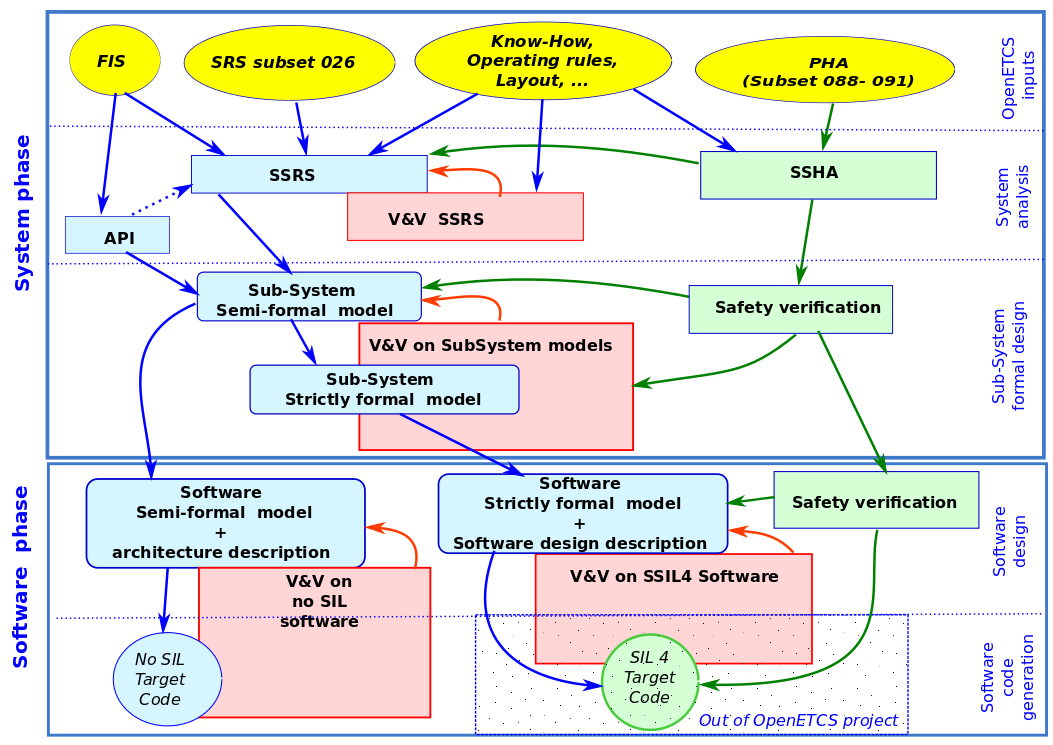
\includegraphics[scale=0.45]{WholeProcess.png}}
  \caption{Main OpenETCS process}
  \label{fig:main_process}
\end{figure}

Yellow elements are inputs, blue elements are part of the design process, red elements are verification and validation activities, green elements are safety activities. Each line (between dash or full blue lines) is a phase of the process, with a name on the right. 

The second section of this document provides a template to describe the means and tools and a list of criteria according WP2 requirements on language, models and tools. The objectives of this description and criteria are to allow to determine the best means of description and associated tool for a given activities.

The third section resumes the results of the evaluation at the end of the benchmark activities.

In Appendix, a section is dedicated to each models produced during the benchmark activities :
\begin{itemize}
\item  CORE
\item  GOPRR
\item  ERTMSFormalSpecs
\item  SysML with Papyrus
\item  SysML with Entreprise Architect
\item  SCADE
\item  EventB with Rodin
\item  Classical B with Atelier B
\item  Petri Nets
\item  System C
\item  GNATprove
\end{itemize}

For each approach and tool, the initial  author of the evaluation is the partner in charge of the modelling. Two assessors, for each approaches,  are in charge of the review of the evaluation and can correct it or add comments.

Tool platform are not covered by this document but in an other output of WP7 :  O7.1.9 "Evaluation of each tool platform against WP2 requirements, independent of target tools".
Besides, Task 7.1 is focussing on design activities : despite that some means can provide verification artefacts for example,  tools and means for validation, verification, test generation,... are in the scope of task 2 and will be analysed later.



%% Bibliography
%\nocite{*}
\bibliographystyle{unsrt}
\bibliography{wp7_bibliography}
%\bibliography{process}

\chapter{Template Description}
\label{sec:template}

\begin{description}
\item[\textcolor{green}{Author}] Author of the approaches description  \todo{Name -  Company}
\item[\textcolor{blue}{Assessor 1}] First assessor of the approaches \todo{Name - Company}
\item[\textcolor{magenta}{Assessor 2}] Second assessor of the approaches \todo{Name - Company}
\end{description}

In the sequel, main text is under the responsibilities of the author.

\begin{author_comment}
Author can add comments using this format at any place.
\end{author_comment}

\begin{assessor1}
First assessor can add comments using this format at any place.
\end{assessor1}

\begin{assessor2}
Second assessor can add comments using this format at any place.
\end{assessor2}

When a note is required, please follow this list :
\begin{description}
\item[0] not recommended, not adapted, rejected
\item[1] weakly recommended, adapted after major improvements, weakly rejected
\item[2] recommended, adapted (with light improvements if necessary)  weakly accepted
\item[3] highly recommended, well adapted,strongly accepted
\item[*] difficult to evaluate with a note (please add a comment under the table)
\end{description}

All the notes can be commented under each table.

\section{Presentation}

This section gives a quick presentation of the tool.

\begin{description}
\item[Name] \todo{Name of the approach and the tool}
\item[Web site] \todo{if available, how to  find information}
\item[License] \todo{Kind of license}
\end{description}

\paragraph{Abstract} Short abstract on the approach and tool (10 lines max)

\paragraph{Publications} Short list of publications on the approach (5 max)

\section{Use and usage of  of the Tool}
According WP2 requirements, give a note for characteristics of the use of the tool (from 0 to 3) :

\begin{tabular}{|l | c | c | c | c|}
\hline
& \textcolor{green}{Author} & \textcolor{blue}{Assessor 1} & \textcolor{magenta}{Assessor 2} & Total \\
\hline 
Open Source (D2.6-02-074) & & & &  \\
\hline 
Cooperation of tools (D2.6-02-076) & & & &  \\
\hline
Robustness (D2.6-02-078) & & & & \\
\hline
Modularity (D2.6-02-078.01) & & & & \\
\hline
Documentation management (D.2.6-02-078.02) & & & & \\
\hline
Distributed software development (D.2.6-02-078.03)  & & & & \\
\hline
Simultaneous Multi-users (D.2.6-02-078.04)   & & & & \\
\hline
Issue tracking (D.2.6-02-078.05) & & & & \\
\hline
Concurrent version development (D.2.6-02-078.08) & & & & \\
\hline
Model-based version control (D.2.6-02-078.09) & & & & \\
\hline
Role traceability (D.2.6-02-078.10) & & & & \\
\hline
Safety version traceability (D.2.6-02-078.11) & & & & \\
\hline
Scalability & & & & \\
\hline
\end{tabular}

The next table resume the capabilities of the tool platform.
\begin{enumerate}
\item Easy integration of a new tool in the tool platform.
\item How expert should we be ?
\item Mechanism for maintaining the tools within the tool platform.
\item Mechanism for bug tracking the tools within the tool platform.
\item Mechanism for updating the tools within the tool platform.
\end{enumerate}

\begin{tabular}{|l | c | c | c | c|}
\hline
& \textcolor{green}{Author} & \textcolor{blue}{Assessor 1} & \textcolor{magenta}{Assessor 2} & Total \\
\hline Easy integration of a new tool &
  &                 &                  &\\
\hline Expertise &
  &                 &                  &\\
\hline Maintenance &
  &                 &                  &\\
\hline Bug tracking &
  &                 &                  &\\
\hline Update &
  &                 &                  &\\
\hline
\end{tabular}

\section{Platform integration}
Capabilities of the tool platform to  be integrated to common operating systems.
\begin{enumerate}
\item  The tools chain shall be portable to common \gls{OS}.
\item   The tool chain shall run stable on all main \gls{OS}.
\item  The tool chain shall run with a good performance on all main \gls{OS}.
\item  Data produce on an \gls{OS} should be readable by an other \gls{OS}.
\end{enumerate}
\begin{tabular}{|l | c | c | c | c|}
  \hline
  & \textcolor{green}{Author} & \textcolor{blue}{Assessor 1} &  \textcolor{magenta}{Assessor 2} & Total \\
  \hline  Portable (R-WP2/D2.6-02-076) &
  &                 &                  &\\
  \hline   Stable (R-WP2/D2.6-02-076.01)&
  &                 &                  &\\
  \hline   Same performance (R-WP2/D2.6-02-076.02)&
  &                 &                  &\\
  \hline  Easy exchange (R-WP2/D2.6-02-076)&
  &                 &                  &\\
  \hline
\end{tabular}


\section{Data integration}
How the tool platform supports the data integration ?

\subsection{How to share data ?}
\begin{enumerate}
\item Files contains all info and are read/write when needed.
\item A central repository contains all data (maybe distributed in a
  set of files).
\item A common database is shared among tools
\item Tools communicate via messages.
\item A meta-model is defined to harmonized the data input/output
\item Representational State Transfer (REST), distributed architecture (like the web) and data access by an
  unique identifier (URL-like).
\end{enumerate}
\begin{tabular}{|l | c | c | c | c|} \hline
  & \textcolor{green}{Author} & \textcolor{blue}{Assessor 1} &  \textcolor{magenta}{Assessor 2} & Total \\
  \hline File based sharing &
  &                 &                  &\\
  \hline Shared repository &
  &                 &                  &\\
  \hline Database based sharing&
  &                 &                  &\\
  \hline Message Passing&
  &                 &                  &\\
  \hline Meta-Model based sharing &
  &                 &                  &\\
  \hline REST architecture style &
  &                 &                  &\\
  \hline
\end{tabular}


\subsection{Data definition}
\begin{enumerate}
\item Definition of a common data format
\item All possible input and output formats of a tool have to be
  documented.
\item Automatic parser/generator support compliant with a common format.
\item Open data formats shall be used for data exchange.
 
\end{enumerate}

\begin{tabular}{|l | c | c | c | c|} \hline
  & \textcolor{green}{Author} & \textcolor{blue}{Assessor 1} &  \textcolor{magenta}{Assessor 2} & Total \\
  \hline Common data format&
  &                 &                  &\\
  \hline Common data format documentation(R-WP2/D2.6-02-076.01) &
  &                 &                  &\\
  \hline Generator/parser &
  &                 &                  &\\
  \hline Open data format (R-WP2/D2.6-02-076.02)&
  &                 &                  &\\
  \hline
\end{tabular}

{\bf Does the tool platform define mechanisms to check the data produces
by a tool ?}

\section{Presentation integration}
The tool chain would be easier to use if the tool may share a common
"look and fell'.
\begin{enumerate}
\item The tool platform proposes a common \gls{GUI}.
\item The tool platform proposes some presentation guidelines
\item The tool platform provides a user interface creation toolkit
\item The tool platform integrates new tools as plug-in of the \gls{IDE}.
\end{enumerate}

\begin{tabular}{|l | c | c | c | c|} \hline
  & \textcolor{green}{Author} & \textcolor{blue}{Assessor 1} &  \textcolor{magenta}{Assessor 2} & Total \\
  \hline Common \gls{GUI}&
  &                 &                  &\\
  \hline Presentation guidelines &
  &                 &                  &\\
  \hline User interface toolkit &
  &                 &                  &\\
  \hline Plug-in support &
  &                 &                  &\\
  \hline
\end{tabular}


\section{Control integration}
The mechanism that allows tools to notify and activate others tools.
\begin{enumerate}
\item Tools may subscribe to some notification.
\item Tools may notify changes.
\item The change may be logged and traced.
\item The tool platform provides a version management.
\item Script based change control.
\end{enumerate}

\begin{tabular}{|l | c | c | c | c|} \hline
  & \textcolor{green}{Author} & \textcolor{blue}{Assessor 1} &  \textcolor{magenta}{Assessor 2} & Total \\
  \hline Service Subscriber&
  &                 &                  &\\
  \hline Service Notifier &
  &                 &                  &\\
  \hline Change traceability &
  &                 &                  &\\
  \hline Version Management &
  &                 &                  &\\
  \hline Script control &
  &                 &                  &\\
  \hline
\end{tabular}


\section{Process integration}
\subsection{Support for engineering process}
Support for a well-defined software engineering process. 
\begin{enumerate}
\item Process definition support.
\item Integrated process : the process is transparent to the users.
\item Process Management support.
\item Script based process: the process is implemented via scripts.
\item The defined tool chain  may be analyzed within the tool platform.
\end{enumerate}

\begin{tabular}{|l | c | c | c | c|} \hline
  & \textcolor{green}{Author} & \textcolor{blue}{Assessor 1} &  \textcolor{magenta}{Assessor 2} & Total \\
  \hline Process Definition &
  &                 &                  &\\
  \hline Process Management &
  &                 &                  &\\
  \hline Integrated Process &
  &                 &                  &\\
  \hline Script based process &
  &                 &                  &\\
  \hline Tool chain Analysis &
  &                 &                  &\\
  \hline
\end{tabular}



\subsection{Support for EN 50128 standard}
Specific mechanism related to EN 50128 standard
\begin{enumerate}
\item  Each tool in the tool chain shall be classified among T1, T2
  and T3 depending on its usage in the process.
\item  For T2 and T3 tools 7 , the choice of tools shall be justified,
  and the justification shall include how the tools failures are
  covered, avoided or taken into account (ref. to EN 50128 6.7.4.2).
\item  All T2 and T3 tools must be provided with their user manuals.
\item  For all T3 tool, the proof of correctness or the measure taken
  to guarantee the correctness of the output w.r.t. their
  specification and the inputs shall be provided. The tool platform
  provides output/input comparison  or other mechanism to guarantee
  the correctness.
\item Does the tool platform provides help to generate or to produce
  documentation about the tool chain such as manual, specification  EN
  50128 §6.7 ?
\item The tool platform helps to define the maintenance process of the
  tool chain.
\item The tool platform provides bug tracker for the tool chain.
\end{enumerate}

\begin{tabular}{|l | c | c | c | c|} \hline
  & \textcolor{green}{Author} & \textcolor{blue}{Assessor 1} &  \textcolor{magenta}{Assessor 2} & Total \\
  \hline Integrated Tools classification (R-WP2/D2.6-02-085)  &
  &                 &                  &\\
  \hline Document production (R-WP2/D2.6-01-042.01) &
  &                 &                  &\\
  \hline Automatic information on tools (R-WP2/D2.6-01-042.02) &
  &                 &                  &\\
  \hline Measure for correctness (R-WP2/D2.6-01-042.03) &
  &                 &                  &\\
  \hline Test of the tool platform &
  &                 &                  &\\
  \hline Tool chain documents  production &
  &                 &                  &\\
  \hline Tool chain maintenance process specification &
  &                 &                  &\\
 \hline Tool chain bug tracker &
  &                 &                  &\\
  \hline
\end{tabular}

\section{Tool chain Analysis}
Is the tool platform able to analyze the tool chain.
\begin{enumerate}
\item The tool platform provides a met-model to represents tool chain
\item The tool platform provides a graphical representation of the
  tool chain
\item The tool platform provides a textual description of the
  tool chain
\item The tool platform may help to analyze the tool chain by means
  of the tools inputs and outputs.
\item The tool platform allows the rearrangement and/or the extension
  of the tool chain
\item Previously define tool chain may be re-use and their confidence too.
\end{enumerate}

\begin{tabular}{|l | c | c | c | c|} \hline
  & \textcolor{green}{Author} & \textcolor{blue}{Assessor 1} &  \textcolor{magenta}{Assessor 2} & Total \\
  \hline Tool chain Meta-Model definition &
  &                 &                  &\\
  \hline Tool chain graphical representation &
  &                 &                  &\\
  \hline Tool chain textual representation &
  &                 &                  &\\
  \hline Tool's Input/output Analysis &
  &                 &                  &\\
  \hline Tool chain Analysis &
  &                 &                  &\\
  \hline Tool chain rearrangement and extension &
  &                 &                  &\\
  \hline Confidence preservation &
  &                 &                  &\\
  \hline
\end{tabular}


\section{Other comments}
Please to  give free comments on the approach.

%%% Local Variables: 
%%% mode: latex
%%% TeX-master: "Evaluation_Platform_against_WP2"
%%% End: 



%% Start here


\chapter{Conclusion}
\label{sec:concl}

This conclusion give a sum up of the evaluation results for each approach. The detailed results of each approach are given in the appendix.

\section{Main usage of the approach}
\label{main_usage}
This section discusses the main usage of the approach.

According to the figure \ref{fig:main_process}, for which phases do you recommend the approach (give a note from 0 to  3) :

\begin{tabular}{|l | c | c | c | c | c | c | c | c | c | c |}
\hline
&  \rotatebox{90}{GOPRR} & \rotatebox{90}{ERTMSFormalSpecs} &  \rotatebox{90}{SysML with Papyrus} &  \rotatebox{90}{SysML with Entreprise Architect} &  \rotatebox{90}{SCADE} &  \rotatebox{90}{EventB} &  \rotatebox{90}{Classical B} & \rotatebox{90}{Petri Nets} &  \rotatebox{90}{System C} &  \rotatebox{90}{GNATprove} \\
\hline 
System Analysis & 5 & & & & & & & & & \\
\hline
Sub-system formal design  & 9 & & & & & & & & & \\
\hline
Software design  & 9 & & & & & & & & & \\
\hline
Software code generation  & 9 & & & & & & & & & \\
\hline
\end{tabular}

According to the figure \ref{fig:main_process}, for which type of activities do you recommend the approach (give a note from 0 to  3) :

\begin{tabular}{|l | c | c | c | c | c | c | c | c | c | c |}
\hline
& \rotatebox{90}{GOPRR} & \rotatebox{90}{ERTMSFormalSpecs} &  \rotatebox{90}{SysML with Papyrus} &  \rotatebox{90}{SysML with Entreprise Architect} &  \rotatebox{90}{SCADE} &  \rotatebox{90}{EventB} &  \rotatebox{90}{Classical B} & \rotatebox{90}{Petri Nets} &  \rotatebox{90}{System C} &  \rotatebox{90}{GNATprove} \\
\hline 
Documentation & 3 & & & & & & & & & \\
\hline
Modeling & 9 & & & & & & & & & \\
\hline
Design  & 6 & & & & & & & & & \\
\hline
Code generation  & 9 & & & & & & & & & \\
\hline
Verification  & 0 & & & & & & & & & \\
\hline
Validation  & 0 & & & & & & & & & \\
\hline
Safety analyses  & 0 & & & & & & & & & \\
\hline
\end{tabular}

\section{Language}
This section discusses the main element of the language.

Which are the main characteristics of the language :

\begin{tabular}{|l | c | c | c | c | c | c | c | c | c | c |}
\hline
& \rotatebox{90}{GOPRR} & \rotatebox{90}{ERTMSFormalSpecs} &  \rotatebox{90}{SysML with Papyrus} &  \rotatebox{90}{SysML with Entreprise Architect} &  \rotatebox{90}{SCADE} &  \rotatebox{90}{EventB} &  \rotatebox{90}{Classical B} & \rotatebox{90}{Petri Nets} &  \rotatebox{90}{System C} &  \rotatebox{90}{GNATprove} \\
\hline 
Informal language & 0 & & & & & & & & & \\
\hline 
Semi-formal language & 0 & & & & & & & & & \\
\hline
Formal language & 8 & & & & & & & & & \\
\hline
Structured language  & 9 & & & & & & & & & \\
\hline
Modular language  & 9 & & & & & & & & & \\
\hline
Textual language  & 0 & & & & & & & & & \\
\hline
Mathematical symbols or code  & 0 & & & & & & & & & \\
\hline
Graphical language  & 9 & & & & & & & & & \\
\hline
\end{tabular}

According WP2 requirements, give a note for the capabilities of the language (from 0 to 3) :

\begin{tabular}{|l | c | c | c | c | c | c | c | c | c | c |}
\hline
& \rotatebox{90}{GOPRR} & \rotatebox{90}{ERTMSFormalSpecs} &  \rotatebox{90}{SysML with Papyrus} &  \rotatebox{90}{SysML with Entreprise Architect} &  \rotatebox{90}{SCADE} &  \rotatebox{90}{EventB} &  \rotatebox{90}{Classical B} & \rotatebox{90}{Petri Nets} &  \rotatebox{90}{System C} &  \rotatebox{90}{GNATprove} \\
\hline
Declarative formalization of properties (D.2.6-X-28)  & 7 & & & & & & & & & \\
\hline
Simple formalization of properties (D.2.6-X-28.1)  & 6 & & & & & & & & & \\
\hline
Scalability : capability to design large model  & 8 & & & & & & & & & \\
\hline
Easily translatable to other languages (D.2.6-X-30)  & 9 & & & & & & & & & \\
\hline
Executable directly (D.2.6-X-33)  & 0 & & & & & & & & & \\
\hline
Executable after translation to a code (D.2.6-X-33)  & 9 & & & & & & & & & \\
(precise if the translation is automatic)  & 8 & & & & & & & & & \\
\hline
Simulation, animation (D.2.6-X-33)  & 0 & & & & & & & & & \\
\hline
Easily understandable (D.2.6-X-27)  & 6 & & & & & & & & & \\
\hline
Expertise level needed (0 High level, 3 few level)  & 6 & & & & & & & & & \\
\hline
Standardization (D.2.6-X-29)  & * & & & & & & & & & \\
\hline
Documented (D.2.6-X-29)  & 7 & & & & & & & & & \\
\hline
Extensible language (D.2.6-01-28)  & 8 & & & & & & & & & \\
\hline
\end{tabular}


\section{System Analysis}
This section discusses the usage of the approach for system analysis.
It can be skipped depending the results of \ref{main_usage}.

Acoording WP2 requirements, how the approach can be involved for the sub-system requirement specification ?

\begin{tabular}{|l | c | c | c | c | c | c | c | c | c | c |}
\hline
& \rotatebox{90}{GOPRR} & \rotatebox{90}{ERTMSFormalSpecs} &  \rotatebox{90}{SysML with Papyrus} &  \rotatebox{90}{SysML with Entreprise Architect} &  \rotatebox{90}{SCADE} &  \rotatebox{90}{EventB} &  \rotatebox{90}{Classical B} & \rotatebox{90}{Petri Nets} &  \rotatebox{90}{System C} &  \rotatebox{90}{GNATprove} \\
\hline
Independent System functions definition (D.2.6-X-10.2.1) & 6 & & & & & & & & & \\
\hline 
System architecture design (D.2.6-X-10.2) & 9 & & & & & & & & & \\
\hline
System data flow identification (D.2.6-X-10.2.3) & 9 & & & & & & & & & \\
\hline
Sub-system focus (D.2.6-X-10.2.4) & 9 & & & & & & & & & \\
\hline
System interfaces definition (D.2.6-X-10.2.5) & 9 & & & & & & & & & \\
\hline
System requirement allocation (D.2.6-X-10.3) & 8 & & & & & & & & & \\
\hline
Traceability with SRS (D.2.6-X-10.5) & 6 & & & & & & & & & \\
\hline
Traceability with Safety activities (D.2.6-X-11) & 6 & & & & & & & & & \\
\hline
\end{tabular}



\section{Sub-System formal design}
This section discusses the usage of the approach for sub-system formal design.
It can be skipped depending the results of \ref{main_usage}.

Two kinds of model can be planned during this phase: semi-formal models to  cover the SSRS (D.2.6-X-12.1) and strictly formal  models to  focuss on some functional and safety aspects (D.2.6-X-14).  Obviously some strictly  formal means can be used to define the semi-formal  model.

\subsection{Semi-formal model}

Concerning semi-formal model, how the WP2 requirements are covered ?

\begin{tabular}{|l | c | c | c | c | c | c | c | c | c | c |}
\hline
& \rotatebox{90}{GOPRR} & \rotatebox{90}{ERTMSFormalSpecs} &  \rotatebox{90}{SysML with Papyrus} &  \rotatebox{90}{SysML with Entreprise Architect} &  \rotatebox{90}{SCADE} &  \rotatebox{90}{EventB} &  \rotatebox{90}{Classical B} & \rotatebox{90}{Petri Nets} &  \rotatebox{90}{System C} &  \rotatebox{90}{GNATprove} \\
\hline 
Consistency to SSRS (D.2.6-X-12.2) & - & & & & & & & & & \\
\hline
Coverage of SSRS (D.2.6-X-12.2.1) & - & & & & & & & & & \\
\hline
Coverage of SSHA (D.2.6-X-12.2.2) & - & & & & & & & & & \\
\hline
Management of requirement justification (D.2.6-X-12.2.3) & - & & & & & & & & & \\
\hline
Traceability to  SSRS (D.2.6-X-12.2.5) & - & & & & & & & & & \\
\hline
Traceability of exported requirements (D.2.6-X-12.2.6) & - & & & & & & & & & \\
\hline
Simulation or animation (D.2.6-X-13 partial) & - & & & & & & & & & \\
\hline
Execution (D.2.6-X-13 partial) & - & & & & & & & & & \\
\hline
Extensible to strictly formal model (D.2.6-X-14.3) & - & & & & & & & & & \\
\hline
Easy to  refine towards strictly formal model (D.2.6-X-14.4) & - & & & & & & & & & \\
\hline
Extensible and modular design (D.2.6-X-15) & - & & & & & & & & & \\
\hline
Extensible to software architecture and design (D.2.6-X-15) & - & & & & & & & & & \\
\hline
\end{tabular}

Concerning safety properties management, how the WP2 requirements are covered ?

\begin{tabular}{|l | c | c | c | c | c | c | c | c | c | c |}
\hline
& \rotatebox{90}{GOPRR} & \rotatebox{90}{ERTMSFormalSpecs} &  \rotatebox{90}{SysML with Papyrus} &  \rotatebox{90}{SysML with Entreprise Architect} &  \rotatebox{90}{SCADE} &  \rotatebox{90}{EventB} &  \rotatebox{90}{Classical B} & \rotatebox{90}{Petri Nets} &  \rotatebox{90}{System C} &  \rotatebox{90}{GNATprove} \\
\hline 
Safety function isolation (D.2.6-X-17) & - & & & & & & & & & \\
\hline 
Safety properties formalisation (D.2.6-X-22) & - & & & & & & & & & \\
\hline
Logical expression (D.2.6-X-28.2.2) & -& & & & & & & & & \\
\hline
Timing constraints (D.2.6-X-28.2.3) & - & & & & & & & & & \\
\hline
Safety properties validation (D.2.6-X-23.2) & - & & & & & & & & & \\
\hline
Logical properties assertion (D.2.6-X-34) & - & & & & & & & & & \\
\hline
Check  of assertions (D.2.6-X-34.1) & - & & & & & & & & & \\
\hline
\end{tabular}

Does the language allow to  formalize (D.2.6-X-31):

\begin{tabular}{|l | c | c | c | c | c | c | c | c | c | c |}
\hline
& \rotatebox{90}{GOPRR} & \rotatebox{90}{ERTMSFormalSpecs} &  \rotatebox{90}{SysML with Papyrus} &  \rotatebox{90}{SysML with Entreprise Architect} &  \rotatebox{90}{SCADE} &  \rotatebox{90}{EventB} &  \rotatebox{90}{Classical B} & \rotatebox{90}{Petri Nets} &  \rotatebox{90}{System C} &  \rotatebox{90}{GNATprove} \\
\hline 
State machines & - & & & & & & & & & \\
\hline
Time-outs & - & & & & & & & & & \\
\hline
Truth tables & - & & & & & & & & & \\
\hline
Arithmetic & - & & & & & & & & & \\
\hline
Braking curves & - & & & & & & & & & \\
\hline
Logical statements & - & & & & & & & & & \\
\hline
Message and fields & - & & & & & & & & & \\
\hline
\end{tabular}


\subsection{Strictly formal model}

Concerning strictly formal model, how the WP2 requirements are covered ?

\begin{tabular}{|l | c | c | c | c | c | c | c | c | c | c |}
\hline
& \rotatebox{90}{GOPRR} & \rotatebox{90}{ERTMSFormalSpecs} &  \rotatebox{90}{SysML with Papyrus} &  \rotatebox{90}{SysML with Entreprise Architect} &  \rotatebox{90}{SCADE} &  \rotatebox{90}{EventB} &  \rotatebox{90}{Classical B} & \rotatebox{90}{Petri Nets} &  \rotatebox{90}{System C} &  \rotatebox{90}{GNATprove} \\
\hline 
Consistency to SFM (D.2.6-X-14.2) & * & & & & & & & & & \\
\hline
Coverage of SSRS (D.2.6-X-14.2) & 3 & & & & & & & & & \\
\hline
Traceability to  SSRS (D.2.6-X-14.3) & 7 & & & & & & & & & \\
\hline
Extensible to software design (D.2.6-X-16) & 3 & & & & & & & & & \\
\hline
Safety function isolation (D.2.6-X-17) & 3 & & & & & & & & & \\
\hline 
Safety properties formalisation (D.2.6-X-22) & 5 & & & & & & & & & \\
\hline
Logical expression (D.2.6-X-28.2.2) & 9 & & & & & & & & & \\
\hline
Timing constraints (D.2.6-X-28.2.3) & 0 & & & & & & & & & \\
\hline
Safety properties validation (D.2.6-X-23.3) & 7 & & & & & & & & & \\
\hline
Logical properties assertion (D.2.6-X-34) & 9 & & & & & & & & & \\
\hline
Proof of assertions (D.2.6-X-34.2) & 8 & & & & & & & & & \\
\hline
\end{tabular}

Does the language allow to  formalize (D.2.6-X-32):

\begin{tabular}{|l | c | c | c | c | c | c | c | c | c | c |}
\hline
& \rotatebox{90}{GOPRR} & \rotatebox{90}{ERTMSFormalSpecs} &  \rotatebox{90}{SysML with Papyrus} &  \rotatebox{90}{SysML with Entreprise Architect} &  \rotatebox{90}{SCADE} &  \rotatebox{90}{EventB} &  \rotatebox{90}{Classical B} & \rotatebox{90}{Petri Nets} &  \rotatebox{90}{System C} &  \rotatebox{90}{GNATprove} \\
\hline 
State machines & 9 & & & & & & & & & \\
\hline
Time-outs & 0 & & & & & & & & & \\
\hline
Truth tables & 0 & & & & & & & & & \\
\hline
Arithmetic & 9 & & & & & & & & & \\
\hline
Braking curves & 9 & & & & & & & & & \\
\hline
Logical statements & 9 & & & & & & & & & \\
\hline
Message and fields & 9 & & & & & & & & & \\
\hline
\end{tabular}


\section{Software design}
This section discusses the usage of the approach for software design.
It can be skipped depending the results of \ref{main_usage}.

\subsection{Functional design}

How the approach allows to  produce a functional software model of the on-board unit ?

\begin{tabular}{|l | c | c | c | c | c | c | c | c | c | c |}
\hline
& \rotatebox{90}{GOPRR} & \rotatebox{90}{ERTMSFormalSpecs} &  \rotatebox{90}{SysML with Papyrus} &  \rotatebox{90}{SysML with Entreprise Architect} &  \rotatebox{90}{SCADE} &  \rotatebox{90}{EventB} &  \rotatebox{90}{Classical B} & \rotatebox{90}{Petri Nets} &  \rotatebox{90}{System C} &  \rotatebox{90}{GNATprove} \\
\hline
Derivation from system semi-formal model & * & & & & & & & & & \\
\hline 
Software architecture description & 9 & & & & & & & & & \\
\hline
Software constraints & 9 & & & & & & & & & \\
\hline
Traceability & 9 & & & & & & & & & \\
\hline
Executable & 8 & & & & & & & & & \\
\hline
\end{tabular}

\subsection{SSIL4 design}

How the approach allows to  produce in safety a software model ?

\begin{tabular}{|l | c | c | c | c | c | c | c | c | c | c |}
\hline
& \rotatebox{90}{GOPRR} & \rotatebox{90}{ERTMSFormalSpecs} &  \rotatebox{90}{SysML with Papyrus} &  \rotatebox{90}{SysML with Entreprise Architect} &  \rotatebox{90}{SCADE} &  \rotatebox{90}{EventB} &  \rotatebox{90}{Classical B} & \rotatebox{90}{Petri Nets} &  \rotatebox{90}{System C} &  \rotatebox{90}{GNATprove} \\
\hline
Derivation from system semi-formal or strictly formal model & * & & & & & & & & & \\
\hline 
Software architecture description & 9 & & & & & & & & & \\
\hline
Software constraints & 9 & & & & & & & & & \\
\hline
Traceability & 9 & & & & & & & & & \\
\hline
Executable & 8 & & & & & & & & & \\
\hline
Conformance to EN50128 § 7.2 & 0 & & & & & & & & & \\
\hline
Conformance to EN50128 § 7.3 & 0 & & & & & & & & & \\
\hline
Conformance to EN50128 § 7.4 & 0 & & & & & & & & & \\
\hline
\end{tabular}

Which criteria for software architecture are covered by the methodology
(see EN50128 table A.3) :

\begin{tabular}{|l | c | c | c | c | c | c | c | c | c | c |}
\hline
& \rotatebox{90}{GOPRR} & \rotatebox{90}{ERTMSFormalSpecs} &  \rotatebox{90}{SysML with Papyrus} &  \rotatebox{90}{SysML with Entreprise Architect} &  \rotatebox{90}{SCADE} &  \rotatebox{90}{EventB} &  \rotatebox{90}{Classical B} & \rotatebox{90}{Petri Nets} &  \rotatebox{90}{System C} &  \rotatebox{90}{GNATprove} \\
\hline
Defensive programming & 7 & & & & & & & & & \\
\hline 
Fault detection \& diagnostic & 7 & & & & & & & & & \\
\hline
Error detecting code & 7 & & & & & & & & & \\
\hline
Failure assertion programming & 9 & & & & & & & & & \\
\hline
Diverse programming & 3 & & & & & & & & & \\
\hline
Memorising executed cases & 0 & & & & & & & & & \\
\hline
Software error effect analysis & 0 & & & & & & & & & \\
\hline
Fully defined interface & 9 & & & & & & & & & \\
\hline
Modelling & 9 & & & & & & & & & \\
\hline
Structured methodology & 9 & & & & & & & & & \\
\hline
\end{tabular}

\section{Software code generation}
This section discusses the usage of the approach for software code generation.
It can be skipped depending the results of \ref{main_usage}.

Which criteria for software design and implementation are covered by the methodology
(see EN50128 table A.4) :

\begin{tabular}{|l | c | c | c | c | c | c | c | c | c | c |}
\hline
& \rotatebox{90}{GOPRR} & \rotatebox{90}{ERTMSFormalSpecs} &  \rotatebox{90}{SysML with Papyrus} &  \rotatebox{90}{SysML with Entreprise Architect} &  \rotatebox{90}{SCADE} &  \rotatebox{90}{EventB} &  \rotatebox{90}{Classical B} & \rotatebox{90}{Petri Nets} &  \rotatebox{90}{System C} &  \rotatebox{90}{GNATprove} \\
\hline
Formal methods & 6* & & & & & & & & & \\
\hline 
Modeling & 6* & & & & & & & & & \\
\hline
Modular approach (mandatory) & 9 & & & & & & & & & \\
\hline
Components & 9 & & & & & & & & & \\
\hline
Design and coding standards (mandatory) & 6* & & & & & & & & & \\
\hline
Strongly typed programming language & 9 & & & & & & & & & \\
\hline

\end{tabular}



\section{Main usage of the tool}
\label{main_usage}

This section discusses the main usage of the tool.

Which task are covered by the tool ?


\begin{tabular}{|l | c | c | c | c | c | c | c | c | c | c |}
\hline
& \rotatebox{90}{GOPRR} & \rotatebox{90}{ERTMSFormalSpecs} &  \rotatebox{90}{SysML with Papyrus} &  \rotatebox{90}{SysML with Entreprise Architect} &  \rotatebox{90}{SCADE} &  \rotatebox{90}{EventB} &  \rotatebox{90}{Classical B} & \rotatebox{90}{Petri Nets} &  \rotatebox{90}{System C} &  \rotatebox{90}{GNATprove} \\
\hline 
Modelling support & 9 & & & & & & & & & \\
\hline
Automatic translation   & 3 & & & & & & & & & \\
\hline
Code Generation   & 9 & & & & & & & & & \\
\hline
Model verification  & 6 & & & & & & & & & \\
\hline
Test generation  & * & & & & & & & & & \\
\hline
Simulation, execution, debugging  & 6 & & & & & & & & & \\
\hline
Formal proof  & 0 & & & & & & & & & \\
\hline
\end{tabular}


\section{Use of the tool}

\begin{tabular}{|l | c | c | c | c | c | c | c | c | c | c |}
\hline
& \rotatebox{90}{GOPRR} & \rotatebox{90}{ERTMSFormalSpecs} &  \rotatebox{90}{SysML with Papyrus} &  \rotatebox{90}{SysML with Entreprise Architect} &  \rotatebox{90}{SCADE} &  \rotatebox{90}{EventB} &  \rotatebox{90}{Classical B} & \rotatebox{90}{Petri Nets} &  \rotatebox{90}{System C} &  \rotatebox{90}{GNATprove} \\
\hline 
Open Source (D2.6-X-36) & 0 & & & & & & & & & \\
\hline 
Portability to operating systems (D2.6-X-37) & 9 & & & & & & & & & \\
\hline
Cooperation of tools (D2.6-X-38) & 3 & & & & & & & & & \\
\hline
Robustness (D2.6-X-41)  & 6* & & & & & & & & & \\
\hline
Modularity (D2.6-X-41.1)  & 0 & & & & & & & & & \\
\hline
Documentation management (D.2.6-X-41.2)  & 0 & & & & & & & & & \\
\hline
Distributed software development (D.2.6-X-41.3)   & 9 & & & & & & & & & \\
\hline
Simultaneous multi-users (D.2.6-X-41.4)   & 9 & & & & & & & & & \\
\hline
Issue tracking (D.2.6-X-41.5)  & 0 & & & & & & & & & \\
\hline
Differences between models (D.2.6-X-41.6)  & 0 & & & & & & & & & \\
\hline
Version management (D.2.6-X-41.7)  & 3 & & & & & & & & & \\
\hline
Concurrent version development (D.2.6-X-41.8)  & 0 & & & & & & & & & \\
\hline
Model-based version control (D.2.6-X-41.9)  & 0 & & & & & & & & & \\
\hline
Role traceability (D.2.6-X-41.10)  & 0 & & & & & & & & & \\
\hline
Safety version traceability (D.2.6-X-41.11)  & 0 & & & & & & & & & \\
\hline
Model traceability (D.2.6-01-035) & 3 & & & & & & & & & \\
\hline
Tool chain integration  & 6* & & & & & & & & & \\
\hline
Scalability  & 6* & & & & & & & & & \\
\hline
\end{tabular}

\section{Certifiability}

This section discusses how the tool can be classified according EN50128 requirements (D.2.6-X-50).


\begin{tabular}{|l | c | c | c | c | c | c | c | c | c | c |}
\hline
& \rotatebox{90}{GOPRR} & \rotatebox{90}{ERTMSFormalSpecs} &  \rotatebox{90}{SysML with Papyrus} &  \rotatebox{90}{SysML with Entreprise Architect} &  \rotatebox{90}{SCADE} &  \rotatebox{90}{EventB} &  \rotatebox{90}{Classical B} & \rotatebox{90}{Petri Nets} &  \rotatebox{90}{System C} &  \rotatebox{90}{GNATprove} \\
\hline 
Tool manual (D.2.6-01-42.02) & 9 & & & & & & & & & \\
\hline
Proof of correctness (D.2.6-01-42.03)    & 0 & & & & & & & & & \\
\hline
Existing industrial  usage  & 9 & & & & & & & & & \\
\hline
Model verification  & 3 & & & & & & & & & \\
\hline
Test generation  & 0 & & & & & & & & & \\
\hline
Simulation, execution, debugging  & 0 & & & & & & & & & \\
\hline
Formal proof  & 0 & & & & & & & & & \\
\hline
\end{tabular}





\appendix



%===================================================
%Do NOT change anything below this line

\end{document}
